 Eventual Consistency ist eine abgeschwächte Variante der Konsistenz, die häufig bei verteilten Datenbanken zur Anwendung kommt. Dabei verzichtet man aus Performancegründen bei Schreiboperationen darauf, Daten sofort auf alle Server/Partitionen zu verteilen.
Stattdessen kommen Algorithmen zum Einsatz, die sicherstellen, dass nach Beendigung der Schreiboperationen die Daten konsistent gemacht werden, in der Regel ohne Aussage darüber, in welchem Zeitraum der Vorgang abgeschlossen sein wird. In der Zwischenzeit sind unterschiedliche Datenbestände auf den einzelnen Servern. Das kann dazu führen, dass identische, zeitgleiche Abfragen von mehreren Benutzern unterschiedliche Ergebnisse liefern können. Man kann lediglich darauf vertrauen, dass die Daten letztendlich konsistent sind, daher der Name diese Konzeptes.
\gls{CAP} Theorem?
\begin{figure}[H]
  \centering
  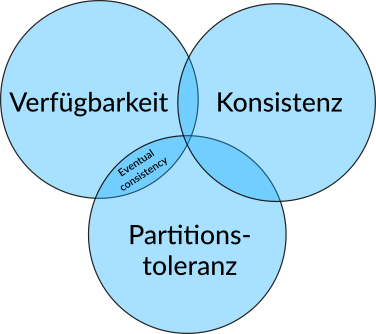
\includegraphics[width=0.6\textwidth]{cap}
  \grayRule
  \caption{Das CAP Theorem}
  \label{fig:cap}
\end{figure}